%!TEX root = *.tex
%%%%%%%%%%%%%%%%%%
% メモ
\begin{comment}

\end{comment}
% カウンタのリセット
% 解答
\qSentence{【解答】}

{
\hang{(1)(a)}
レンツの法則より,X$\rightarrow$Yの向きに誘導電流が流れるので,
コンデンサーのs側極板の電荷$Q$は正である.
また,時刻$t$における誘導起電力の大きさは$lvB$である.\hfill

\begin{wrapfigure}{r}{12zw}
  \vspace{-\intextsep}
  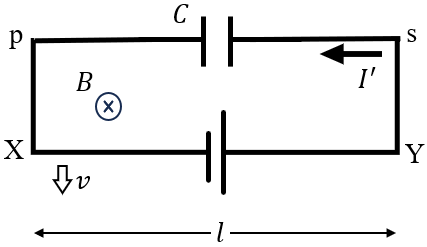
\includegraphics[width=12zw]{../graphs/jumon_134_sol_1.png}
\end{wrapfigure}

\begin{align*}
  Q &= +C(lvB) = ClvB
\end{align*}

\hang{\qquad (b)}
(a)と同様に考えると,
\begin{align*}
  Q+\Delta Q &= Cl(v+\Delta v)B \\
  \Delta Q &= ClB\Delta v 
\end{align*}
\sethang{(1)(b)}\noindent
であるので,
\begin{align*}
  I^\prime &= \dfrac{\Delta Q}{\Delta t} 
  = \dfrac{ClB\Delta v}{\Delta t} \\
  &= ClBa
\end{align*}

\par}


{
\hang{(2)}
$\Delta t$の間に流れる電流$I$が$\Delta I$だけ変化したとき,
コイルに生じる誘導起電力は$-L\tfrac{\Delta I}{\Delta t}$である.
\begin{wrapfigure}{r}{12zw}
  \vspace{-\intextsep}
  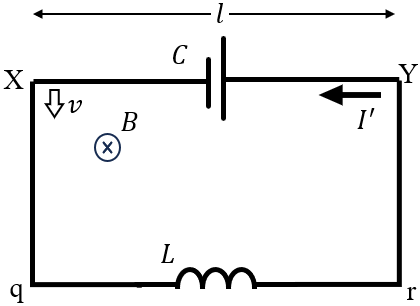
\includegraphics[width=12zw]{../graphs/jumon_134_sol_2.png}
\end{wrapfigure}

キルヒホッフの法則より
\begin{align*}
  lvB - L\dfrac{\Delta I}{\Delta t} &= 0 \\
  lB\dfrac{\Delta x}{\Delta t} &= L\dfrac{\Delta I}{\Delta t} \\
  \therefore\ \dfrac{\Delta I}{\Delta x} &= \dfrac{lB}{L}
\end{align*}
\par}

\sethang{(2)}
$\tfrac{\Delta I}{\Delta x}$が定数ということは,$I$は$x$の一次式で表されるということである.
時刻$t=0$において$x=0,\,I=0$なので
\begin{align*}
  I &= \dfrac{lB}{L}x
\end{align*}

\hang{(3)}
導体棒にはX$\rightarrow$Yの向きに電流$(I+I^\prime)$が流れているので,
電流が磁場から受ける力$l(I+I^\prime)B$が鉛直上向きにはたらく.
運動方程式より
\begin{align*}
  Ma = Mg - l(I+I^\prime)B
\end{align*}

\hang{(4)}
(3)の運動方程式に(1)(b)と(2)の結果を代入すると,
\begin{align*}
  Ma &= Mg - l\left(\dfrac{lB}{L}x\right)B - l(ClBa)B \\
  (M+Cl^2B^2) a &= Mg - \dfrac{l^2B^2}{L}x \\
  \therefore\ a &= -\dfrac{l^2B^2}{L(M+Cl^2B^2)} \left(x-\dfrac{MgL}{l^2B^2}\right)
\end{align*}
が得られる.
これより導体棒は
角振動数$\omega = \tfrac{lB}{\sqrt{L(M+Cl^2B^2)}}$
で単振動をし,
振動中心の座標$x_0$は$x_0=\tfrac{MgL}{l^2B^2}$である。

\hang{(5)}
$t=0$で$x=0$であるから,単振動の振幅は$x_0$である.
よって,導体棒の動く範囲は$0\leqq x\leqq 2x_0$である.
コイルを流れる電流$I$の最大値と最小値を$I_{\rm min},I_{\rm max}$とすると
\begin{align*}
  I_{\rm min} &= 0 \\
  I_{\rm max} &= \dfrac{lB}{L}\cdotp \dfrac{2MgL}{l^2B^2} = \dfrac{2Mg}{lB}
\end{align*}

%%%%%%%%%%%%%%%%%%